\documentclass[14pt]{extbook}
\usepackage{multicol, enumerate, enumitem, hyperref, color, soul, setspace, parskip, fancyhdr} %General Packages
\usepackage{amssymb, amsthm, amsmath, latexsym, units, mathtools} %Math Packages
\everymath{\displaystyle} %All math in Display Style
% Packages with additional options
\usepackage[headsep=0.5cm,headheight=12pt, left=1 in,right= 1 in,top= 1 in,bottom= 1 in]{geometry}
\usepackage[usenames,dvipsnames]{xcolor}
\usepackage{dashrule}  % Package to use the command below to create lines between items
\newcommand{\litem}[1]{\item#1\hspace*{-1cm}\rule{\textwidth}{0.4pt}}
\pagestyle{fancy}
\lhead{Progress Quiz 5}
\chead{}
\rhead{Version A}
\lfoot{8497-6012}
\cfoot{}
\rfoot{Summer C 2021}
\begin{document}

\begin{enumerate}
\litem{
Solve the equation below. Then, choose the interval that contains the solution.\[ -12(7x + 16) = -8(19x -10) \]\begin{enumerate}[label=\Alph*.]
\item \( x \in [1.3, 2.6] \)
\item \( x \in [2.8, 4.9] \)
\item \( x \in [-2, -1.3] \)
\item \( x \in [-1.1, 1.2] \)
\item \( \text{There are no real solutions.} \)

\end{enumerate} }
\litem{
Write the equation of the line in the graph below in Standard Form $Ax+By=C$. Then, choose the intervals that contain $A, B, \text{ and } C$.
\begin{center}
    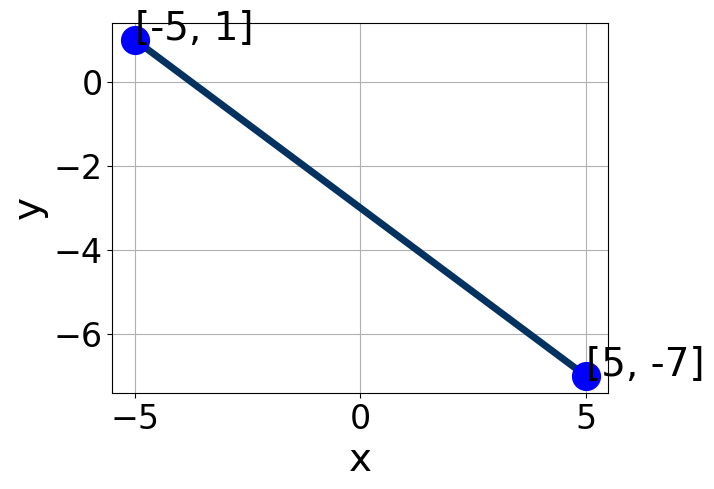
\includegraphics[width=0.5\textwidth]{../Figures/linearGraphToStandardCopyA.png}
\end{center}
\begin{enumerate}[label=\Alph*.]
\item \( A \in [-6.2, -3.8], \hspace{3mm} B \in [-6.6, -4], \text{ and } \hspace{3mm} C \in [14, 17] \)
\item \( A \in [1.8, 4.5], \hspace{3mm} B \in [3.4, 5.6], \text{ and } \hspace{3mm} C \in [-15, -14] \)
\item \( A \in [-1.7, 3.2], \hspace{3mm} B \in [-3.6, -0.6], \text{ and } \hspace{3mm} C \in [1, 7] \)
\item \( A \in [1.8, 4.5], \hspace{3mm} B \in [-6.6, -4], \text{ and } \hspace{3mm} C \in [14, 17] \)
\item \( A \in [-1.7, 3.2], \hspace{3mm} B \in [0.5, 2], \text{ and } \hspace{3mm} C \in [-7, 0] \)

\end{enumerate} }
\litem{
Solve the equation below. Then, choose the interval that contains the solution.\[ -11(-6x -15) = -16(13x -8) \]\begin{enumerate}[label=\Alph*.]
\item \( x \in [1.86, 2.31] \)
\item \( x \in [-0.16, 0.17] \)
\item \( x \in [-1.34, -0.84] \)
\item \( x \in [0.74, 1.35] \)
\item \( \text{There are no real solutions.} \)

\end{enumerate} }
\litem{
Solve the linear equation below. Then, choose the interval that contains the solution.\[ \frac{5x -7}{4} - \frac{-7x + 3}{5} = \frac{5x -4}{2} \]\begin{enumerate}[label=\Alph*.]
\item \( x \in [1.4, 3.3] \)
\item \( x \in [-5.7, -5.3] \)
\item \( x \in [37.3, 40.8] \)
\item \( x \in [-0.6, 0.6] \)
\item \( \text{There are no real solutions.} \)

\end{enumerate} }
\litem{
First, find the equation of the line containing the two points below. Then, write the equation in the form $ y=mx+b $ and choose the intervals that contain $m$ and $b$.\[ (8, 7) \text{ and } (-4, -8) \]\begin{enumerate}[label=\Alph*.]
\item \( m \in [-4.2, -0.9] \hspace*{3mm} b \in [-13.99, -12.84] \)
\item \( m \in [-0.7, 3.4] \hspace*{3mm} b \in [-5.93, -3.61] \)
\item \( m \in [-0.7, 3.4] \hspace*{3mm} b \in [1.04, 3.61] \)
\item \( m \in [-0.7, 3.4] \hspace*{3mm} b \in [-1.64, 0.07] \)
\item \( m \in [-0.7, 3.4] \hspace*{3mm} b \in [-3.33, -2.61] \)

\end{enumerate} }
\litem{
Find the equation of the line described below. Write the linear equation in the form $ y=mx+b $ and choose the intervals that contain $m$ and $b$.\[ \text{Parallel to } 6 x - 5 y = 7 \text{ and passing through the point } (9, 3). \]\begin{enumerate}[label=\Alph*.]
\item \( m \in [1.14, 1.5] \hspace*{3mm} b \in [-10.2, -6.2] \)
\item \( m \in [0.54, 1.14] \hspace*{3mm} b \in [-10.2, -6.2] \)
\item \( m \in [1.14, 1.5] \hspace*{3mm} b \in [-6.9, -5.9] \)
\item \( m \in [-1.23, -0.79] \hspace*{3mm} b \in [13.5, 15.2] \)
\item \( m \in [1.14, 1.5] \hspace*{3mm} b \in [6.6, 8.7] \)

\end{enumerate} }
\litem{
Solve the linear equation below. Then, choose the interval that contains the solution.\[ \frac{5x -6}{5} - \frac{8x + 3}{4} = \frac{-9x + 5}{7} \]\begin{enumerate}[label=\Alph*.]
\item \( x \in [47, 53] \)
\item \( x \in [7.32, 11.32] \)
\item \( x \in [0.44, 3.44] \)
\item \( x \in [3.07, 6.07] \)
\item \( \text{There are no real solutions.} \)

\end{enumerate} }
\litem{
First, find the equation of the line containing the two points below. Then, write the equation in the form $ y=mx+b $ and choose the intervals that contain $m$ and $b$.\[ (-6, 10) \text{ and } (-11, -10) \]\begin{enumerate}[label=\Alph*.]
\item \( m \in [1, 12] \hspace*{3mm} b \in [-38, -33] \)
\item \( m \in [1, 12] \hspace*{3mm} b \in [32, 38] \)
\item \( m \in [1, 12] \hspace*{3mm} b \in [15, 18] \)
\item \( m \in [-7, -2] \hspace*{3mm} b \in [-54, -48] \)
\item \( m \in [1, 12] \hspace*{3mm} b \in [-4, 6] \)

\end{enumerate} }
\litem{
Write the equation of the line in the graph below in Standard Form $Ax+By=C$. Then, choose the intervals that contain $A, B, \text{ and } C$.
\begin{center}
    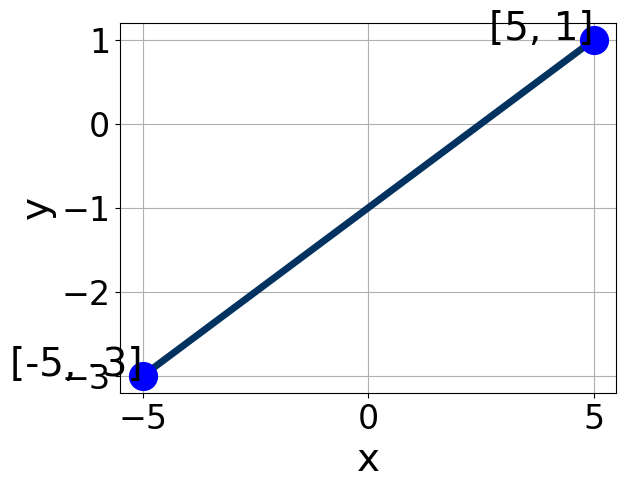
\includegraphics[width=0.5\textwidth]{../Figures/linearGraphToStandardA.png}
\end{center}
\begin{enumerate}[label=\Alph*.]
\item \( A \in [-1.6, 0.3], \hspace{3mm} B \in [0.5, 1.4], \text{ and } \hspace{3mm} C \in [-2.3, 0.75] \)
\item \( A \in [-1.6, 0.3], \hspace{3mm} B \in [-3.1, 0.8], \text{ and } \hspace{3mm} C \in [0.97, 1.79] \)
\item \( A \in [1, 2.5], \hspace{3mm} B \in [4.4, 5.7], \text{ and } \hspace{3mm} C \in [-5.13, -4.33] \)
\item \( A \in [-3.9, -1.4], \hspace{3mm} B \in [4.4, 5.7], \text{ and } \hspace{3mm} C \in [-5.13, -4.33] \)
\item \( A \in [1, 2.5], \hspace{3mm} B \in [-6.2, -4.9], \text{ and } \hspace{3mm} C \in [3.89, 6.19] \)

\end{enumerate} }
\litem{
Find the equation of the line described below. Write the linear equation in the form $ y=mx+b $ and choose the intervals that contain $m$ and $b$.\[ \text{Parallel to } 4 x + 3 y = 3 \text{ and passing through the point } (8, -5). \]\begin{enumerate}[label=\Alph*.]
\item \( m \in [-1.67, -0.87] \hspace*{3mm} b \in [-14, -7] \)
\item \( m \in [-1.67, -0.87] \hspace*{3mm} b \in [-5.67, -2.67] \)
\item \( m \in [1.1, 1.75] \hspace*{3mm} b \in [-20.67, -13.67] \)
\item \( m \in [-0.95, -0.37] \hspace*{3mm} b \in [2.67, 6.67] \)
\item \( m \in [-1.67, -0.87] \hspace*{3mm} b \in [2.67, 6.67] \)

\end{enumerate} }
\end{enumerate}

\end{document}